\scanpage{39}
\deleted{\unsure{Soit}}

Soit $K$ un corps topologique isomorphe à $\mathbf C$, $X$ un schéma algébrique défini sur $K$. Alors $X_{\mathrm{top}}$ est défini, et aussi $H^*(X_{\mathrm{top}},K)$. D'autre part, \inserted{si $X$ est non sing.,} la cohomologie de Hodge est définie, \unsure{soit} $H^*(X)$ [indépendant de la structure topologique de $K$]. Alors le choix d'un isom top. $u:K\unsure{-|\longrightarrow}\mathbf C$ définit un isomorphisme
\[
H^*(X_{\mathrm{top}},K)\xrightarrow{\sim}H^*(X)
\]
et on vérifie aussitôt que cet isomorphisme ne dépend pas du choix de $u$. [En d'autres termes, si $K=\mathbf C$, alors les deux homomorphismes
\diagram{\begin{tikzcd}[ampersand replacement=\&,column sep=large,row sep=large]
\& H^*(X)\arrow[dd,"{\text{(antilinéaire)}}"]\\
H^*(X_{\mathrm{top}},\mathbf C)\arrow[ur]\arrow[dr]\arrow[phantom,r,"{\text{non comm.}}"{description,xshift=-6pt}]
 \& {}\\
\& H^*(X^c)
\end{tikzcd}}
(où $c:\mathbf C\unsure{-|\longrightarrow}\mathbf C$ est la conjugaison complexe) sont \deleted{conjugués} déduits l'un de l'autre par application de $c$ aux coefficients dans $H^*(X_{\mathrm{top}},\mathbf C)$]

\inserted{Cela nous permet, notant qu'on a un \unsure{isom injectif|hom injectif} continu unique $u:\mathbf R\to\mathbf C$, de définir $H^*(X_{\mathrm{top}},\mathbf R)\hookrightarrow H^*(X)$ (même si $X$ pas définissable sur $\mathbf R$ !) d'où une sous-\inserted{$\mathbf R$-}algèbre de $H^*(X)$, \deleted{\unsure{définie sur $\mathbf R$}} notée $H^*(\unsure{X_{\mathrm{top}}|X},\mathbf R)$ \deleted{$H^*(X)^{\unsure{+}}$} \deleted{\unsure{cela indépendant de la topologie de $K$}}, on obtient $H^*(X)^-=\sqrt{-1}H^*(X)^+$}

\figure{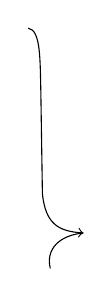
\begin{tikzpicture}[x=1cm,y=1cm]
\draw[->] (0,2.7) .. controls (.16,2.68) and (.15,2.3) .. (.16,1.9) -- (.18,.6) .. controls (.22,.2) and (.4,.12) .. (.7,.1);
\draw (.28,-.35) .. controls (.22,-.1) and (.4,.07) .. (.7,.1);
\end{tikzpicture}}

Supposons $X$ projective non \uline{singulière}, alors le choix d'un isom top. $u:K\xrightarrow{\sim}\mathbf C$ définit une décomposition
\[
\varphi:\coprod_{p,q}H^q(X,\Omega_X^p)\xrightarrow{\sim}H^*(X)
\]
compatible avec la filtration de $H^*(X)$. On vérifie encore que $\varphi$ est indépendant du choix de $u$.
\mspage{38}
